\documentclass[border=3pt]{standalone}
\usepackage{tikz}
\usetikzlibrary{decorations.pathreplacing,patterns}
\definecolor{greengreen}{rgb}{0.0, 0.42, 0.24}
%%%%%%%%%%%%%%%%%%%%%%%%%%%%%%%%%%%%%%%%%%%%%%%%%%%%%%%%%%%%%%%%%
\begin{document}
%%%%%%%%%%%%%%%%%%%%%%%%%%%%%%%%%%%%%%%%%%%%%%%%%%%%%%%%%%%%%%%%%
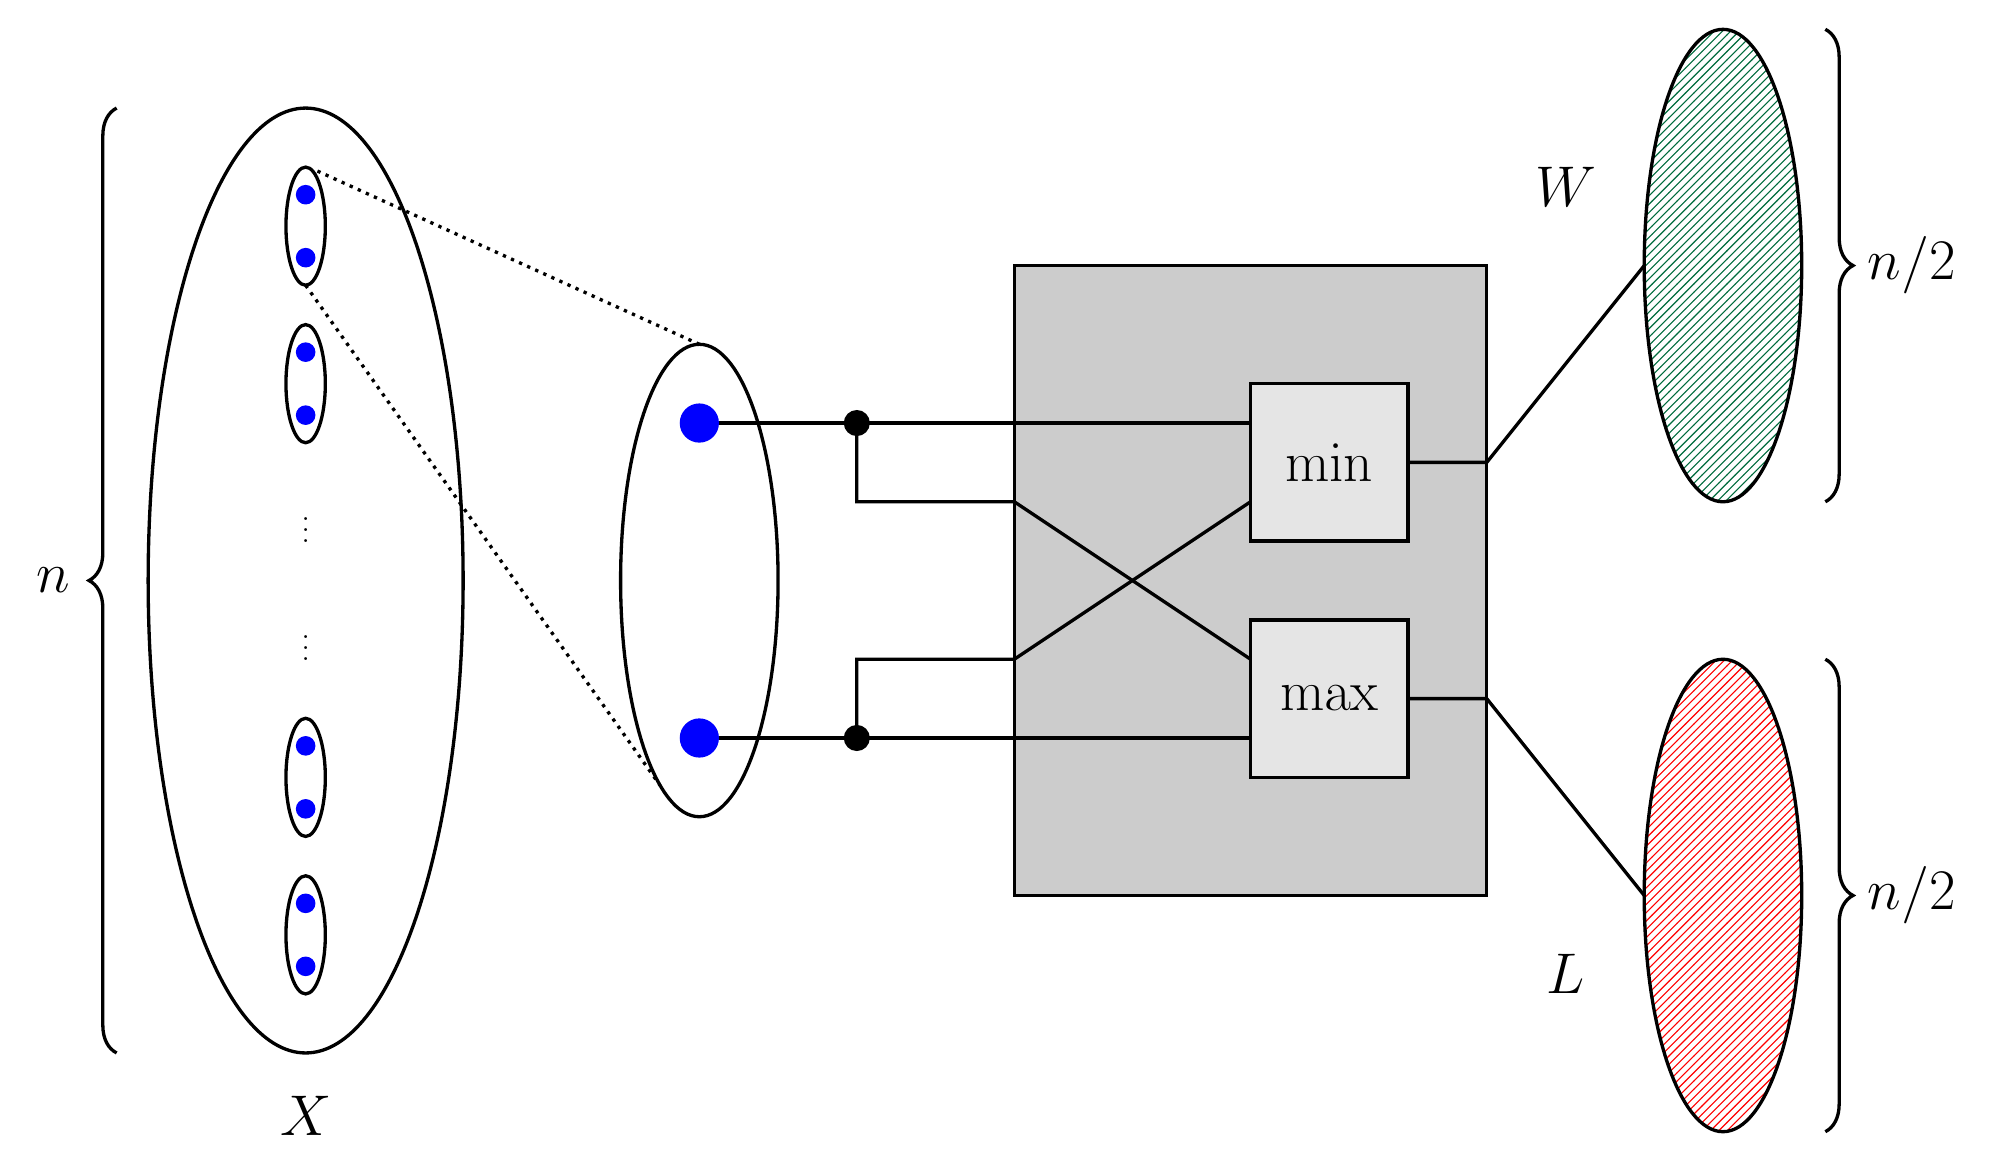
\begin{tikzpicture}[blue/.style={fill=blue,very thick,circle,inner sep=0pt}]
%================================================================
%	Left Ellipse
\draw[very thick] (0,0) ellipse (2cm and 6cm);
%----------------------------------------------------------------
\draw[very thick] (0,4.5) ellipse (.25cm and .75cm);
\draw[very thick] (0,-4.5) ellipse (.25cm and .75cm);
\draw[very thick] (0,2.5) ellipse (.25cm and .75cm);
\draw[very thick] (0,-2.5) ellipse (.25cm and .75cm); 
%----------------------------------------------------------------
\node[style = blue, text width = .25cm] at (0,4.1) {};
\node[style = blue, text width = .25cm] at (0,4.9) {};
\node[style = blue, text width = .25cm] at (0,2.1) {};
\node[style = blue, text width = .25cm] at (0,2.9) {};
\node[style = blue, text width = .25cm] at (0,-4.1) {};
\node[style = blue, text width = .25cm] at (0,-4.9) {};
\node[style = blue, text width = .25cm] at (0,-2.1) {};
\node[style = blue, text width = .25cm] at (0,-2.9) {};
%----------------------------------------------------------------
\node[thick] at (0,.75) {$\vdots$};
\node[thick] at (0,-.75) {$\vdots$};
\node at (0, -6.8) {\huge $X$};
\draw[very thick, decorate,decoration={brace,amplitude=10pt}] (-2.4,-6) -- (-2.4,6);
\node at (-3.2,0) {\huge $n$};

%================================================================
%	Box
\draw[very thick, color=black, fill = gray!40] (9,-4) rectangle (15,4);
\draw[very thick, color=black, fill = gray!20] (12,0.5) rectangle (14,2.5);
\draw[very thick, color=black, fill = gray!20] (12,-0.5) rectangle (14,-2.5);
%----------------------------------------------------------------
\node at (13,1.5) {\huge $\min$};
\node at (13,-1.5) {\huge $\max$};

%================================================================
%	Lines
\draw[very thick] (5,2) -- (12,2);
\draw[very thick] (5,-2) -- (12,-2);
\node[very thick, circle, fill=black] at (7,2) {};
\node[very thick, circle, fill=black] at (7,-2) {};
\draw[very thick] (7,2) -- (7,1) -- (9,1) -- (12,-1);
\draw[very thick] (7,-2) -- (7,-1) -- (9,-1) -- (12,1);
\draw[very thick] (14,1.5) -- (15,1.5) -- (17,4);
\draw[very thick] (14,-1.5) -- (15,-1.5) -- (17,-4);

%================================================================
%	Center Ellipse
\draw[very thick] (5,0) ellipse (1cm and 3cm);
%----------------------------------------------------------------
\node[style = blue, text width = .5cm] at (5,2) {};
\node[style = blue, text width = .5cm] at (5,-2) {};
%----------------------------------------------------------------
\draw[very thick, dotted] (0.15,5.2) -- (5,3);
\draw[very thick, dotted] (0,3.75) -- (4.5,-2.6);

%================================================================
%	Right Ellipses
\draw[very thick,pattern=north east lines, pattern color=greengreen] (18,4) ellipse (1cm and 3cm);
\draw[very thick,pattern=north east lines, pattern color=red] (18,-4) ellipse (1cm and 3cm);
%----------------------------------------------------------------
\draw[very thick, decorate,decoration={brace,amplitude=10pt, mirror}] (19.3,1) -- (19.3,7);
\draw[very thick, decorate,decoration={brace,amplitude=10pt,mirror}] (19.3,-7) -- (19.3,-1);
\node at (20.4,4) {\huge $n/2$};
\node at (20.4,-4) {\huge $n/2$};
\node at (16,5) {\huge $W$};
\node at (16,-5) {\huge $L$};
%================================================================
\end{tikzpicture}
%%%%%%%%%%%%%%%%%%%%%%%%%%%%%%%%%%%%%%%%%%%%%%%%%%%%%%%%%%%%%%%%%
\end{document}
%%%%%%%%%%%%%%%%%%%%%%%%%%%%%%%%%%%%%%%%%%%%%%%%%%%%%%%%%%%%%%%%%